\documentclass[journal]{IEEEtran}
\usepackage[T1]{fontenc}
\usepackage[utf8]{inputenc}
\usepackage{amsmath,amssymb}
\usepackage{graphicx}
\usepackage{booktabs}
\usepackage{multirow}
\usepackage{cite}
\usepackage{microtype}

\newcommand{\code}[1]{{\small #1}}

% Plain abstract/keywords labels (no em dash); body text not bold/italic.
\makeatletter
\renewenvironment{abstract}{%
  \normalfont\normalsize
  \par\noindent\textbf{Abstract:}\space
}{%
  \par\vspace{0.5\baselineskip}%
}
\renewenvironment{IEEEkeywords}{%
  \normalfont\normalsize
  \par\noindent\textbf{Index Terms:}\space
}{%
  \par\vspace{0.5\baselineskip}%
}
% Run-in paragraph headings (e.g. Discussion a/b/c) in roman, not IEEEtran italic.
\renewcommand\paragraph{\@startsection{paragraph}{4}{0pt}%
  {1.5ex \@plus 1.5ex \@minus 0.5ex}%
  {-1em}%
  {\normalfont\normalsize}}
\makeatother

\hyphenation{agentic work-flows fore-casting Context-Optimizer}

\begin{document}

\title{Task-Aware Token Budget Forecasting for Agentic Workflows}

\author{Harish~Gaggar, Intuit Inc., Email: harish\_gaggar@intuit.com}

\markboth{}{}

\maketitle

\begin{abstract}
Agentic large language model (LLM) workflows interleave model calls, tools, and
growing conversation state, routinely consuming far more tokens than single-turn
chat. Teams still size context reactively, which raises cost and risks
context-window failures. This paper asks whether the task description available
at dispatch time is sufficient to forecast per-stage token use before execution.
Task-Aware Budget Forecaster (TABF) extracts lexical signals, classifies task
type and complexity, and predicts a per-stage budget without any LLM call. A
gradient-boosted regressor trained on simulated traces raises the
within-twenty-percent rate from 65.4\% to 74.1\% on a six-hundred-task
reproducible benchmark (McNemar $p=0.009$). ContextOptimizer trims live message
lists before each model call while preserving tool-call/response structure; on
public multi-turn trace fixtures it reduced measured input tokens by 72\%
across fourteen instrumented evaluation calls. Real-trace holdout evaluation and persona
fixtures illustrate limits of synthetic transfer and motivate coupling
forecasting to runtime trimming.
\end{abstract}

\begin{IEEEkeywords}
Agent-based systems, natural language processing, machine learning, knowledge-based systems, applications.
\end{IEEEkeywords}

\section{Impact Statement}
Agentic AI systems bill inference by conversation length and tool
output, yet budgets are often static defaults. Accurate pre-flight token forecasts
enable cost gates, model routing, and capacity planning before expensive
multi-step runs start. In-loop trimming that preserves tool protocols can cut
recurring input spend without adding another model call inside the optimiser path.
Together, forecasting and structured compression address a growing share of AI
operating expenditure and reduce out-of-context failures in customer-facing
workflows. Reproducible benchmarks let practitioners compare methods on equal
footing.

\section{Introduction}
\label{sec:intro}

LLM agents now run in production with context windows from 128K to 1M tokens,
while aggregate prompt length has grown rapidly with multi-step
workflows~\cite{aubakirova2025}. Reactive budgeting uses generous defaults plus
mid-session compaction and degrades quality through context
rot~\cite{hong2025}, compounds billable tokens~\cite{tokalator2026}, and
complicates service-level planning. Much of the eventual consumption is
foreshadowed in the dispatch-time task text (tool verbs, file references,
comparison language, multi-step connectives), which motivates treating budgeting
as structured prediction rather than post-hoc truncation.

The paper contributes: (i)~a five-stage formulation of agentic token budgets;
(ii)~TABF, a linear-time forecaster with interpretable rules and an optional
gradient-boosted trees (GBT) tier; (iii)~a seeded open benchmark with byte-stable
replay; (iv)~ContextOptimizer, an in-loop funnel with tool-pairing invariants;
(v)~evaluations on public traces and synthetic personas with explicit observational
limits.

\section{Related Work}
\label{sec:related}

Context engineering spans retrieval, compression, memory, and tool-augmented
reasoning~\cite{mei2025,mohsenimofidi2025}. Runtime budget methods include
BudgetThinker~\cite{wen2025}, tree-search allocation~\cite{li2025budget}, and
SWE-Pruner~\cite{wang2025swepruner}. CompactPrompt~\cite{wang2025compactprompt}
and Tool Attention~\cite{sadani2026} reduce prompt or schema bulk at inference
time; both differ from multi-turn message trimming with hard tool invariants.
ACE~\cite{zhang2025ace} and hierarchical policies~\cite{taparia2026} adapt
context using training signal or online feedback, whereas TABF's heuristic tier
needs no traces. Tokenomics~\cite{salim2025} motivates task-type-dependent stage
costs; EGTP~\cite{xie2026egtp} predicts output length from hidden states and
requires model access. Trace-centric suites such as AI-NativeBench~\cite{wang2026ainativebench}
attribute cost post-hoc; TABF targets lightweight pre-flight estimates when
traces do not yet exist.

\section{Problem Formulation}
\label{sec:problem}

An agent executing task $\tau$ consumes tokens across system prompt $S$, tool
schema $T$, working memory $M$, retrieved context $C$, reasoning $R$, and output
$O$. Total consumption is $B(\tau)=\sum$ stages. The forecasting task is to
estimate $\hat{B}(\tau)=(\hat{S},\ldots,\hat{O})$ before execution. Intermediate
labels are task type $\kappa(\tau)$ and complexity $\delta(\tau)\in$
\{\textsc{low},\textsc{medium},\textsc{high},\textsc{expert}\}. The primary
metric is within-20\% rate (W20R): fraction of held-out tasks with
$|\hat{B}-B|/B\le 0.20$, supplemented by mean absolute error (MAE) and mean
absolute percentage error (MAPE) on totals.

\section{The TABF Framework}
\label{sec:framework}

TABF is a four-stage pipeline: signal extraction, rule-based classification,
budget model (heuristic or GBT), and a serialisable \code{BudgetForecast}
object with per-stage estimates, confidence, and method tag. The pipeline is
$O(|\tau|)$ and makes no LLM call.

\subsection{Signal extractor and classifier}
The extractor maps $\tau$ to $\sigma(\tau)\in\mathbb{R}^8$ using regular
expressions only: word count; five keyword-family indicators (multi-step,
tools, code, files, comparisons); question count; and a coarse entity proxy.
The classifier applies priority-ordered rules on $\sigma$ to assign $\kappa$ and
$\delta$, disambiguating overlapping templates (e.g., code keywords plus HTTP
verbs without multi-step language route to \textsc{code\_generation} rather than
\textsc{tool\_use\_chain}). On the evaluation split, agreement with latent
labels is 95.1\% (type), 86.5\% (complexity), 83.2\% (both).

\subsection{Heuristic and GBT budget models}
The heuristic indexes per-type base allocations calibrated on 240 tasks and
scales them by complexity ($0.65$--$2.4\times$). A word-count adjustment inflates
retrieved context for long prompts. With traces, two GBT regressors predict total
input and output tokens from ten hand features (eight signals plus type and
complexity indices); per-stage splits reuse heuristic ratios for stability
(\code{n\_estimators=120}, \code{max\_depth=4}, \code{learning\_rate=0.08}).
Table~\ref{tab:base} lists medium-complexity heuristic bases (LOW/HIGH/EXPERT
scale columns by $0.65$--$2.4\times$).

\begin{table*}[!t]
\caption{Heuristic per-stage base allocations at MEDIUM complexity (tokens).}
\label{tab:base}
\centering
\footnotesize
\begin{tabular}{lrrrrrr}
\toprule
Task type & Sys. & Tools & Mem. & Ctx. & Reas. & Out. \\
\midrule
Code generation & 800 & 600 & 400 & 1200 & 1800 & 1200 \\
Bug fix & 800 & 500 & 600 & 2000 & 2200 & 800 \\
Refactoring & 800 & 500 & 800 & 2500 & 2500 & 1500 \\
Documentation & 600 & 200 & 300 & 1500 & 800 & 2000 \\
Multi-step plan & 900 & 800 & 700 & 1500 & 2800 & 1200 \\
Data analysis & 700 & 700 & 500 & 3000 & 2000 & 1500 \\
Research query & 600 & 1200 & 400 & 3500 & 1500 & 1000 \\
Tool-use chain & 800 & 1500 & 600 & 2000 & 2000 & 800 \\
\bottomrule
\end{tabular}
\end{table*}

\section{Experimental Setup}
\label{sec:setup}

Public per-stage traces are scarce; evaluation uses an open synthetic benchmark:
600 tasks across eight types, 15\% complexity jitter and 7\% type swaps on latent
labels, and a log-normal simulator with signal-dependent residuals invisible to
the heuristic. Corpus seed 1729, simulator seed 20260514, stratified 415/415
train/test split (seed 42), GBT \code{random\_state=0}. Shared rule machinery
makes synthetic W20R optimistic; oracle-label and real-trace evaluations bound
leakage and transfer error.

Baselines include uniform train mean (B1), type-only lookup (B2), length slope
(B3), and Ridge/RandomForest/HistGradientBoosting on hand features or TF-IDF
1--2grams (B4--B8). McNemar tests ($\alpha=0.05$, exact, two-sided) compare
W20R against TABF+GBT.

\section{Results}
\label{sec:results}

Table~\ref{tab:main} reports held-out accuracy ($n=185$). TABF+GBT achieves
74.05\% W20R (MAE 1882, MAPE 15.9\%), improving over the 65.4\% heuristic
($p=0.009$) and more than doubling naive uniform allocation. RandomForest and
HistGB on the same features are statistically tied (McNemar $p=1.0$) but lack
per-stage decomposition and a zero-training tier. TF-IDF HistGB reaches 69.7\%
W20R without task-type rules, bounding text-only approaches.

\begin{table*}[!t]
\caption{Main results ($n=185$). McNemar $p$ vs.\ TABF+GBT.}
\label{tab:main}
\centering
\footnotesize
\setlength{\tabcolsep}{4pt}
\begin{tabular}{lrrrr}
\toprule
Method & MAE & MAPE (\%) & W20R (\%) & $p$ \\
\midrule
B1: Uniform & 4497 & 50.2 & 28.1 & $<10^{-4}$ \\
B2: Type-only & 4839 & 36.2 & 30.3 & $<10^{-4}$ \\
B3: Length-proportional & 3982 & 38.4 & 34.1 & $<10^{-4}$ \\
B4: Ridge (hand) & 2289 & 21.7 & 55.7 & $10^{-5}$ \\
B5: RandomForest (hand) & 1883 & 15.9 & 74.1 & 1.000 \\
B6: HistGB (hand) & 1877 & 15.9 & 73.5 & 1.000 \\
B7: Ridge (TF-IDF) & 1890 & 17.3 & 64.3 & 0.003 \\
B8: HistGB (TF-IDF) & 2037 & 17.5 & 69.7 & 0.169 \\
TABF heuristic & 2503 & 18.2 & 65.4 & 0.009 \\
\textbf{TABF + GBT} & \textbf{1882} & \textbf{15.9} & \textbf{74.1} & n/a \\
\bottomrule
\end{tabular}
\end{table*}

\begin{figure}[!t]
\centering
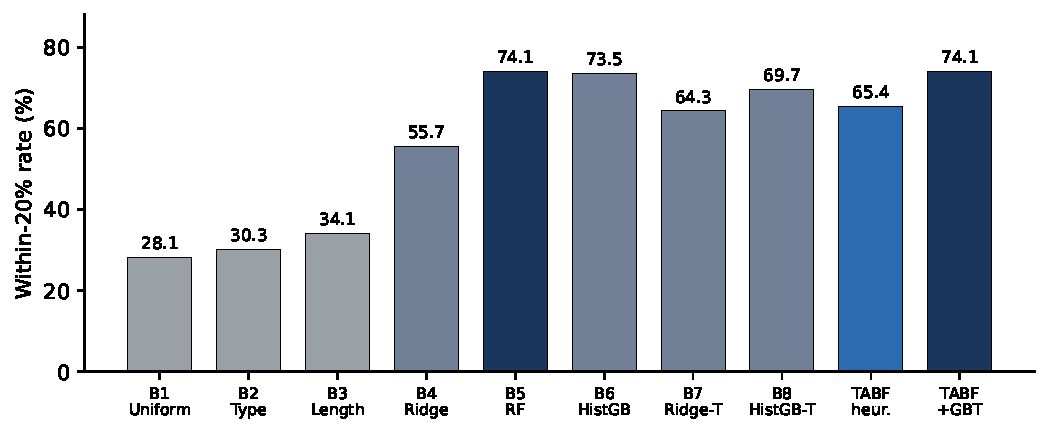
\includegraphics[width=\linewidth]{results/fig_w20r.pdf}
\caption{Within-20\% rate by method.}
\label{fig:w20r}
\end{figure}

\begin{figure}[!t]
\centering
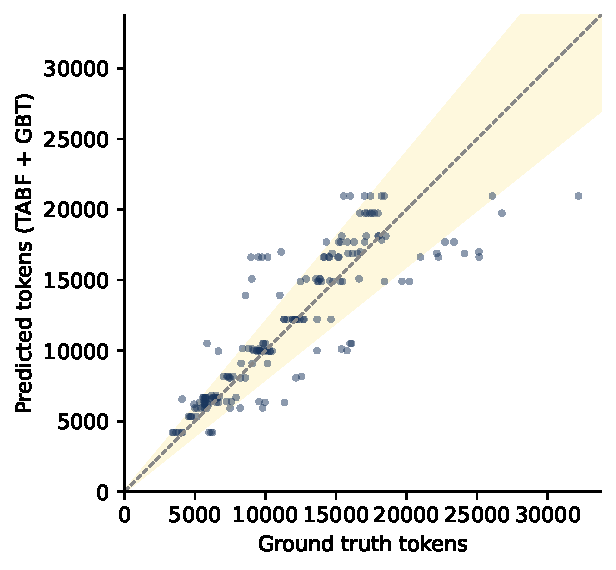
\includegraphics[width=0.48\linewidth]{results/fig_calibration.pdf}
\hfill
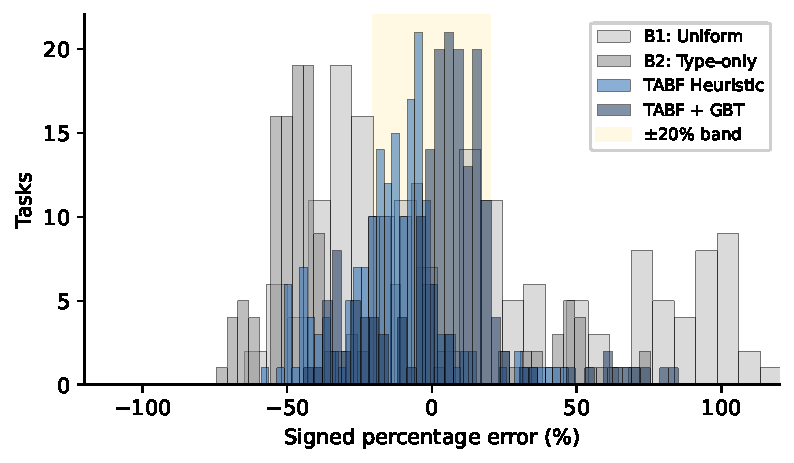
\includegraphics[width=0.48\linewidth]{results/fig_error_dist.pdf}
\caption{Predicted vs.\ true tokens (left) and error histograms (right) for TABF+GBT.}
\label{fig:calib}
\end{figure}

\begin{figure}[!t]
\centering
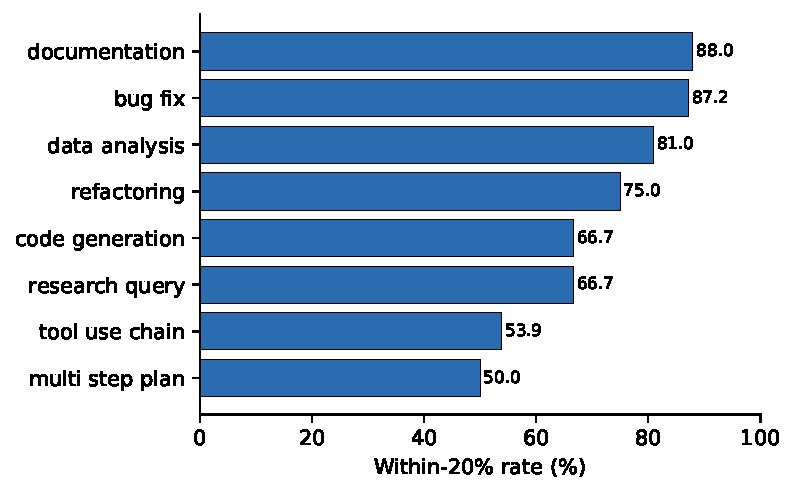
\includegraphics[width=\linewidth]{results/fig_per_type_w20r.pdf}
\caption{TABF+GBT W20R by latent task type.}
\label{fig:pertype}
\end{figure}

Fig.~\ref{fig:pertype} ranks W20R by latent task type. Bug-fix and documentation
reach 87--88\%; tool-use chains and multi-step plans lag (53--50\%, $n=8$ for the
latter). Ablations confirm
complexity scaling is critical ($-$34.6~pp W20R when flattened to
\textsc{medium}); code-keyword and entity-count removals cost 10--12~pp.

\begin{table}[!t]
\caption{Selected heuristic ablations.}
\label{tab:ablation}
\centering
\footnotesize
\begin{tabular}{lrr}
\toprule
Configuration & W20R (\%) & $\Delta$ pp \\
\midrule
Full heuristic & 65.4 & n/a \\
$-$ complexity scaling & 30.8 & $-$34.6 \\
$-$ code keywords & 55.1 & $-$10.3 \\
$-$ entity count & 57.3 & $-$8.1 \\
\bottomrule
\end{tabular}
\end{table}

\paragraph{Robustness.}
Five-seed cross-validation yields $71.7\pm4.0\%$ W20R for TABF+GBT. Dedicated
per-stage GBT models raise mean stage W20R from 53.6\% to 62.9\% (+9.3~pp) with
nearly unchanged total W20R (73.5\% vs.\ 74.1\%). Oracle latent labels inflate
GBT W20R by only +2.2~pp versus +10.8~pp for the heuristic
(Table~\ref{tab:oracle}). Training on 63 real agent turns and testing on 20
reaches 25.0\% W20R with train-median calibration; synthetic TABF+GBT without
scaling stays near 6.0\% on the same corpus (Table~\ref{tab:real}).

\begin{table}[!t]
\caption{Oracle vs.\ predicted labels (synthetic test).}
\label{tab:oracle}
\centering
\footnotesize
\begin{tabular}{lrr}
\toprule
Model & Predicted & Oracle \\
\midrule
TABF heuristic W20R (\%) & 63.2 & 74.1 \\
TABF + GBT W20R (\%) & 71.4 & 73.5 \\
\bottomrule
\end{tabular}
\end{table}

\begin{table}[!t]
\caption{Real-trace holdout (public evaluation corpus).}
\label{tab:real}
\centering
\footnotesize
\begin{tabular}{lrr}
\toprule
Setting & $n_\text{test}$ & W20R (\%) \\
\midrule
Trained 63 / test 20 & 20 & 25.0 \\
Synthetic TABF+GBT & 83 & 6.0 \\
\bottomrule
\end{tabular}
\end{table}

\section{ContextOptimizer}
\label{sec:optimizer}

TABF addresses dispatch-time allocation; ContextOptimizer trims the live
message list before each LLM call. Layers fall into four categories executed in
fixed order: (i)~\textbf{compression} deduplicates tool results and large file
payloads; (ii)~\textbf{reranking} scores segments with BM25 or recency heuristics;
(iii)~\textbf{selection} enforces a token budget on retained segments;
(iv)~\textbf{clustering} merges repeated tool-call patterns (e.g., polling).
Adapters map LangChain, OpenAI chat, or plain dict messages; tool-call/response
pairing is a hard invariant so OpenAI-compatible agents do not break. Presets
trade aggressiveness: \code{minimal} (compression only), \code{balanced}
(compression + BM25/recency + budget selector, 8K cap), and \code{aggressive}
(adds clustering). The default \code{balanced} preset performs no internal LLM
call, keeping optimiser latency near tens of milliseconds on median agent-shaped
inputs.

\section{Trace and Persona Evaluation}
\label{sec:production}

ContextOptimizer is evaluated on released public multi-turn traces and synthetic
personas (TABF remains offline). Fourteen instrumented evaluation calls show 72.0\% input-token reduction
(215{,}438 $\to$ 60{,}250; best ratio 0.12). An 83-turn population averages
27{,}757 input tokens (median 22{,}382; p95 64{,}922). Projecting the measured
reduction yields ${\approx}$20K saved input tokens per turn; at 1{,}000 turns/day
illustrative annual input savings are \$1{,}094 (gpt-4o-mini), \$18{,}236
(gpt-4o), and \$21{,}883 (claude-sonnet-4.5) at May 2026 list prices
(Table~\ref{tab:prodcost}).

\begin{table}[!t]
\caption{Trace evaluation savings and projected annual cost (@ 1k turns/day, input only).}
\label{tab:prodcost}
\centering
\footnotesize
\begin{tabular}{lr}
\toprule
Metric & Value \\
\midrule
Reduction (14 calls) & 72.0\% \\
Eval turns $N$ & 83 \\
Median latency (complete) & 26.5\,s \\
Status complete (\%) & 77.1 \\
\bottomrule
\end{tabular}
\end{table}

\begin{figure}[!t]
\centering
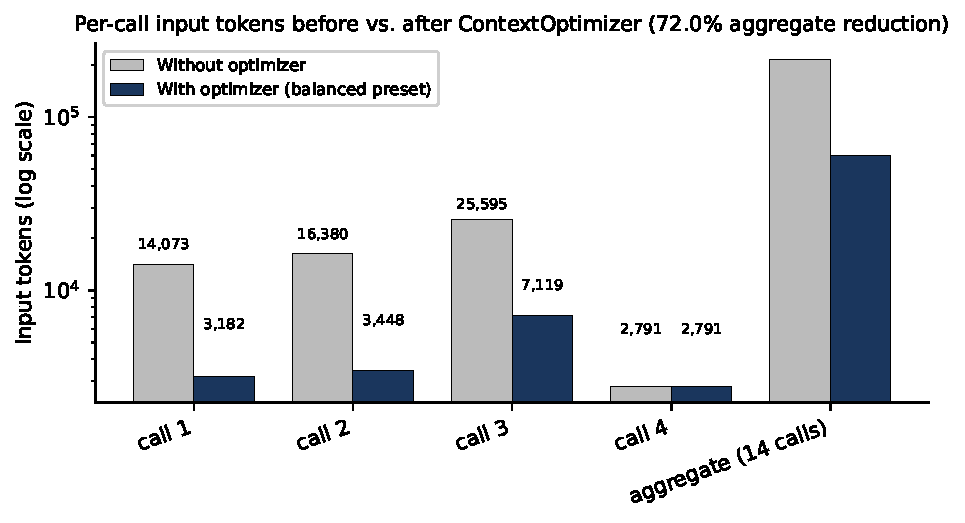
\includegraphics[width=\linewidth]{results/fig_production_savings.pdf}
\caption{Per-call input tokens before/after optimiser (log scale).}
\label{fig:prod}
\end{figure}

A 100-run microbenchmark on agent-shaped synthetic inputs reports median
49\,ms overhead per call (p95 529\,ms at 449K tokens). Four personas (25 seeds
each) average 70.0\% reduction; training-free truncation (B9) overshoots on long
RAG threads while ContextOptimizer wins on duplicate reads and polling
(Table~\ref{tab:personas}; Fig.~\ref{fig:personas}).

\begin{figure}[!t]
\centering
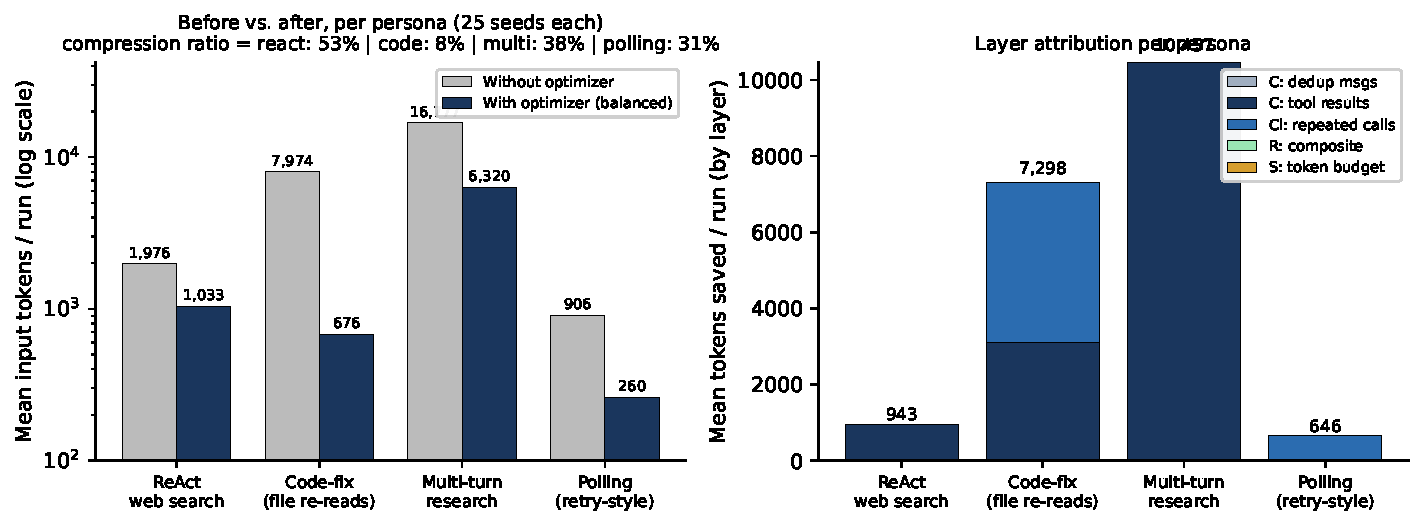
\includegraphics[width=\linewidth]{results/fig_generic_agents.pdf}
\caption{Persona benchmark: tokens before/after and layer attribution.}
\label{fig:personas}
\end{figure}

\begin{table}[!t]
\caption{Persona means (\% input reduction, 25 seeds).}
\label{tab:personas}
\centering
\footnotesize
\begin{tabular}{lrr}
\toprule
Persona & B9 & ContextOptimizer \\
\midrule
ReAct web search & 42.2 & 47.7 \\
Code-fix & 3.5 & 91.5 \\
Multi-turn research & 92.9 & 62.3 \\
Polling & 0.0 & 71.3 \\
\bottomrule
\end{tabular}
\end{table}

\section{Discussion}
\label{sec:discussion}

\paragraph{Forecasting.}
Headline synthetic W20R should be read as an in-house upper bound: latent labels
and TABF inputs share rule chains, and English keyword features may fail on
multilingual or domain-specific jargon. Oracle-label experiments show GBT gains
are not primarily label leakage (+2.2~pp). The authoritative generalisation test
is real-trace training: 25\% W20R after calibration vs.\ 6\% zero-shot transfer,
indicating per-deployment scale factors or ${\sim}100$ local traces before
unattended budget gates. Five-seed CV ($71.7\pm4.0\%$) and stress perturbations
(2$\times$ reasoning mass, shuffled stage ratios) show learned models near 71--74\%
W20R while the heuristic collapses when ratios are wrong; fixed tables must be
recalibrated per agent topology.

\paragraph{Optimisation.}
Trace-replay savings (72\% over fourteen calls) are direct measurements from the
public evaluation package, not modelled. The 83-turn corpus contextualises scale but does not substitute
for a randomised quality A/B against an unoptimised control; 77.1\% task-complete
status is observational. Persona and B9 baselines are synthetic; CompactPrompt-
style compression on live multi-turn logs remains future work. Tool-schema
middleware such as Tool Attention is complementary to post-hoc pruning layers.

\paragraph{Composition.}
TABF and ContextOptimizer are designed to compose (forecast at dispatch,
enforce in the loop) but are not wired end-to-end: the optimiser still uses a
static \code{max\_tokens}. A closed loop would log (forecast, realised, saved)
for retraining and tighten ceilings over time.

\section{Conclusion}
\label{sec:conclusion}

Agentic token budgeting can be split across pre-flight forecasting and in-loop
trimming without LLM calls inside either default path. TABF places 74.1\% of
synthetic forecasts within $\pm$20\% on a reproducible six-hundred-task benchmark;
ContextOptimizer cut measured input tokens by 72\% on held-out public traces while preserving
tool invariants. Real traces and persona tests clarify where each component
works today and what deployment integration remains. Reproducibility artifacts
accompany this submission as supplementary material for review.

\bibliographystyle{IEEEtran}
\bibliography{paper}

\end{document}
